% arXiv-ready LaTeX source (main.tex)
% ----------------------------------------------------------------------
\documentclass[11pt]{article}
\usepackage[utf8]{inputenc}
\usepackage[T1]{fontenc}
\usepackage{lmodern,microtype,geometry}
\geometry{margin=1in}
\usepackage{amsmath,amssymb,amsthm,mathtools,bm,bbm}
\usepackage{enumitem}
\usepackage[hidelinks]{hyperref}
\usepackage[nameinlink]{cleveref}
\usepackage{graphicx}
\usepackage{booktabs}
\usepackage{xcolor}
\usepackage{float}
\usepackage{siunitx}

% --- Theorem-like envs -------------------------------------------------
\newtheorem{theorem}{Theorem}[section]
\newtheorem{proposition}[theorem]{Proposition}
\newtheorem{lemma}[theorem]{Lemma}
\newtheorem{definition}[theorem]{Definition}
\newtheorem{assumption}[theorem]{Assumption}
\newtheorem{remark}[theorem]{Remark}

% --- Metadata ----------------------------------------------------------
\title{\textbf{A Deterministic Limit Order Book Simulator with Hawkes-Driven Order Flow:}\\
\textbf{Theory, Diagnostics, and Reproducible Benchmarks}}
\author{Sohaib El Karmi\\
\small IMT Atlantique, Brest, France\\
\small \texttt{sohaib.el-karmi@imt-atlantique.net}}
\date{}

% --- Macros ------------------------------------------------------------
\newcommand{\R}{\mathbb{R}}
\newcommand{\E}{\mathbb{E}}
\newcommand{\1}{\mathbbm{1}}
\newcommand{\Law}{\mathcal{L}}
\newcommand{\Norm}[1]{\left\lVert#1\right\rVert}
\newcommand{\ip}[1]{\left\langle #1 \right\rangle}

\begin{document}
\maketitle

\begin{abstract}
We present a reproducible research stack for market microstructure: a modern C++ deterministic limit order book (LOB) engine, a multivariate \emph{marked} Hawkes order-flow generator exposed to both C++ and Python, and a set of diagnostics and benchmarks released with code and artifacts. On the theory side, we recall stability conditions for linear and nonlinear Hawkes processes, provide a correctness argument for Ogata-style thinning, and use the time--rescaling theorem to build goodness-of-fit tests. Empirically, we calibrate and compare exponential vs.\ power-law kernels on \emph{Binance BTCUSDT} trades and \emph{LOBSTER AAPL} Level-X books, reporting likelihood, KS/QQ residuals, ACFs, and branching ratios, with deterministic scripts to regenerate all figures and tables. Our results highlight (i) the practical importance of subcritical but \emph{nearly unstable} regimes for realistic clustering, and (ii) where Hawkes-based simulators match or miss LOB stylized facts relative to queue-reactive baselines. The full stack (code, configs, figures) accompanies this paper.
\end{abstract}

\section{Introduction}
Clustered order arrivals and feedback between trades and future activity are central to high-frequency dynamics. Hawkes processes provide a natural framework for self- and cross-excitation in order flow, yet practical deployments often rely on proprietary data and opaque calibration pipelines. Reproducible, theory-anchored stacks that couple a deterministic LOB core with statistically validated Hawkes generators remain scarce.

\paragraph{Problem statement.} Practitioners need a simulator that (i) obeys price--time priority exactly, (ii) supports classical and heavy-tailed Hawkes dynamics with marks, and (iii) exposes diagnostics that certify whether fitted models capture stylized facts on public datasets. Without such tooling it is difficult to benchmark emerging neural Hawkes or queue-reactive approaches against transparent baselines.

\paragraph{Contributions.}
\begin{enumerate}[leftmargin=*, itemsep=2pt]
  \item \textbf{Deterministic LOB + Hawkes bridge.} We release a C++ engine with a Python bridge that simulates marked multivariate Hawkes order flow directly into the book. The implementation mirrors the theoretical requirements of \cref{sec:stability}, including explicit spectral radius checks and incremental intensity updates used by our thinning sampler.
  \item \textbf{Reproducible calibration suite.} Scripts under \texttt{scripts/} and \texttt{experiments/} calibrate exponential and power-law kernels on Binance BTCUSDT trades and LOBSTER AAPL Level-X messages. Seeds, configuration files, and generated artifacts (JSON metadata, NPZ datasets, figures, tables) are versioned for exact regeneration.
  \item \textbf{Diagnostics and baselines.} We operationalise time-rescaling QQ/KS tests, intensity ACFs, and branching ratio estimates, and we juxtapose Hawkes-driven flows with a deterministic queue-reactive baseline. Section~\ref{sec:results} interprets where each approach matches or deviates from observed clustering.
\end{enumerate}

\paragraph{Roadmap.} \Cref{sec:related} revisits Hawkes and LOB literature with emphasis on reproducible tooling. \Cref{sec:simulator} describes the simulator and its connection to stability theory. \Cref{sec:theory} collects guarantees for existence, thinning, and diagnostics. \Cref{sec:methodology} documents datasets, calibration, and baselines. \Cref{sec:results} reports quantitative results, followed by discussion and limitations in \cref{sec:discussion}. Reproducibility details appear in \cref{sec:repro}.

\section{Background and related work}\label{sec:related}
\subsection{Hawkes processes in market microstructure}
A (linear) multivariate Hawkes process with marks has conditional intensity
\begin{equation}
\lambda_i(t) = \mu_i + \sum_{j=1}^d \sum_{t_k^{(j)}<t} \phi_{ij}\big(t-t_k^{(j)}, V_k^{(j)}\big), \qquad i=1,\dots,d,
\end{equation}
where the kernel $\phi_{ij}$ encodes self- and cross-excitation and $V_k^{(j)}$ are marks (volumes). Empirical finance adopts this framework to model clustered trades, quote updates, and cross-asset spillovers \cite{Bacry2015,ContKukanovStoikov2014}. Neural variants \cite{MeiEisner2017} and transformer backbones \cite{Zuo2020} improve expressivity but rarely integrate with deterministic LOB engines.

\subsection{Stability and nearly-unstable regimes}
For linear Hawkes with integrable kernels, stationarity holds when the spectral radius of the kernel's $L^1$ matrix is strictly less than one \cite{BremaudMassoulie1996}. Nearly-unstable limits ($\rho(G)\uparrow 1$) reproduce long-memory effects \cite{JaissonRosenbaum2015}. Nonlinear Hawkes admit contraction-based stability results given Lipschitz activation functions \cite{BremaudMassoulie1996}. We mirror these conditions in code by checking $\rho(G)$ before simulating and logging branching ratios.

\subsection{Limit order book simulators and baselines}
Markovian queueing models provide tractability for optimal execution \cite{ContLarrard2013}, whereas queue-reactive intensities conditioned on state better match intrabook statistics \cite{HuangLehalleRosenbaum2015}. Public simulators that expose code, calibration scripts, and diagnostics remain limited. The \texttt{tick} library \cite{Tick} supports classical Hawkes estimation, but it does not couple to deterministic LOB engines. Our contribution is a unified stack that bridges these components.

\section{Simulator overview}\label{sec:simulator}
\paragraph{Order book core.} The C++ engine implements price--time priority with submissions, cancellations, and executions as discrete events. State is the queue vector around a reference price; matching is deterministic given an event stream. The implementation records every fill to allow post-hoc risk analysis.

\paragraph{Order flow model.} We consider $d$ event types (market buy/sell, limit at best levels, cancellations). Arrivals follow a $d$-variate marked Hawkes process; marks (volumes) can be log-normal or exponential and scale the excitation. The Python bridge exposes these generators with NumPy arrays for integration in notebooks or Streamlit dashboards.

\paragraph{Kernels.} We use
\begin{align}
\text{Exponential:}\quad & \phi_{ij}(u,v) = \alpha_{ij} v e^{-\beta_{ij} u} \1\{u>0\},\\
\text{Power-law:}\quad & \phi_{ij}(u,v) = \alpha_{ij} v (u+c_{ij})^{-\gamma_{ij}} \1\{u>0\},\quad \gamma_{ij}>1.
\end{align}
Let $G_{ij}=\int_0^\infty \E[\phi_{ij}(u,V)]\,du$ and $G=(G_{ij})$. We expose $\rho(G)$ and branching ratios via the diagnostics JSON files to verify subcriticality.

\section{Theoretical foundations}\label{sec:theory}
\subsection{Existence and stability}\label{sec:stability}
\begin{theorem}[Linear Hawkes stability]
For a linear multivariate Hawkes process with integrable kernels and $G$ as above, if $\rho(G)<1$, then a unique stationary and ergodic version exists; the mean intensity solves $\bm{\Lambda}=(I-G)^{-1}\bm{\mu}$.
\end{theorem}
\begin{proof}[Sketch]
Classical results interpret the process as a Poisson cluster (immigration-birth) system; subcritical branching ($\rho(G)<1$) ensures non-explosion and existence of a stationary solution \cite{BremaudMassoulie1996,DaleyVereJones2003}. Our simulator computes $G$ directly from fitted parameters and aborts runs when $\rho(G)\ge 1$.
\end{proof}

\begin{theorem}[Nonlinear stability via contraction]
Consider a (possibly marked) nonlinear Hawkes $\lambda_i(t)=\psi_i\!\left(\mu_i+\sum_j(\phi_{ij}\ast dN_j)(t)\right)$ with each $\psi_i$ Lipschitz with constant $L_i$ and $\int_0^\infty \E|\phi_{ij}(u,V)|\,du = G_{ij}$. If $\rho(\mathrm{diag}(L)\,G)<1$, then a stationary version exists and is mixing.
\end{theorem}
\begin{proof}[Sketch]
A weighted contraction mapping argument on the intensity trajectory yields existence and uniqueness \cite{BremaudMassoulie1996}. In implementation we bound $L_i$ for sigmoid activations and verify $\rho(\mathrm{diag}(L)G)$ numerically.
\end{proof}

\begin{remark}[Branching ratios]
For linear/marked Hawkes, $n_i=\sum_j G_{ij}$ is the expected number of offspring spawned by type $i$. We report $\hat n$ in \cref{tab:benchmarks} and emit warnings in the simulator when $\hat n>0.95$ to signal nearly-unstable regimes.
\end{remark}

\subsection{Simulation correctness and diagnostics}
\begin{proposition}[Ogata-style thinning]
Let $\bar\lambda(t)$ dominate the (history-dependent) intensity $\lambda(t)$ almost surely. Generate a Poisson process of rate $\bar\lambda$ and accept each candidate at time $T$ with probability $\lambda(T)/\bar\lambda(T)$. The accepted points form a realization with conditional intensity $\lambda$.
\end{proposition}
\begin{proof}[Sketch]
Conditioning on the candidate process, acceptances are independent Bernoulli draws with success probability matching the desired hazard \cite{Ogata1981,LewisShedler1979}. Our C++ implementation maintains exponential kernel states so that $\bar\lambda$ tracks the true intensity tightly, reducing rejections.
\end{proof}

\begin{remark}[Cluster simulation]
For linear Hawkes, immigrants sampled from a homogeneous Poisson process can generate offspring via branching, enabling perfect simulation \cite{MollerRasmussen2005}. We mirror this in tests to validate thinning outputs.
\end{remark}

\begin{proposition}[Time-rescaling residuals]
If $\{T_k\}$ follows a point process with conditional intensity $\lambda(t)$, then the transformed inter-arrivals $U_k=1-\exp\!\left(-\int_{T_{k-1}}^{T_k}\lambda(s)ds\right)$ are i.i.d.\ $\mathrm{Unif}(0,1)$. QQ/KS tests on $\{U_k\}$ assess model fit.
\end{proposition}

\subsection{Nearly-unstable scaling}
When $\Norm{G}\uparrow 1$, rescaled Hawkes counts converge to diffusions (e.g., CIR/Heston-type) \cite{JaissonRosenbaum2015}. This observation motivates targeting $\hat n$ near but below one to emulate heavy clustering while avoiding explosion.

\section{Experimental methodology}\label{sec:methodology}
\subsection{Datasets}
\paragraph{Binance BTCUSDT.} We ingest public trade prints from \cite{BinanceData}. After cleaning with \texttt{scripts/preprocess\_binance.py}, we aggregate one full day (2025-09-21) into buy/sell event streams with volumes and timestamps. The resulting dataset contains \num{945965} events over \num{86399.5} seconds.

\paragraph{LOBSTER AAPL Level-X.} We process the 2012-06-21 sample from \cite{LOBSTER}, reconstruct the level-10 book, and extract market, limit-at-best, and cancel events. Each hour-long window contains approximately \num{150000} events.

\subsection{Calibration pipeline}
\begin{enumerate}[leftmargin=*, itemsep=2pt]
  \item \textbf{Windowing.} We partition event streams into sliding windows (length \SI{3600}{s}, \SI{50}{\percent} overlap) using \texttt{experiments/configs/day14\_binance.yaml}. Burn-in histories of \SI{900}{s} ensure intensity warm-up.
  \item \textbf{Optimization.} Exponential kernels are fitted via L-BFGS with spectral radius penalties (see \texttt{hawkes\_baseline.ipynb}); power-law kernels use truncated likelihoods with gradient clipping. We initialise from queue-agnostic rates derived from empirical intensities.
  \item \textbf{Diagnostics.} \texttt{scripts/collect\_runs.py} aggregates split metrics, while \texttt{scripts/prepare\_summary\_assets.py} recomputes calibration curves, branching ratios, and publishes CSV/PNG artifacts.
\end{enumerate}

\subsection{Queue-reactive baseline}
We implement a deterministic queue-reactive model following \cite{HuangLehalleRosenbaum2015}: intensities depend on current queue depths at best bid/ask and are calibrated via maximum likelihood on the same windows. The baseline operates without self-excitation (branching ratio zero) and serves as a sanity check for Poisson-type arrivals.

\section{Results}\label{sec:results}
\begin{figure}[H]
  \centering
  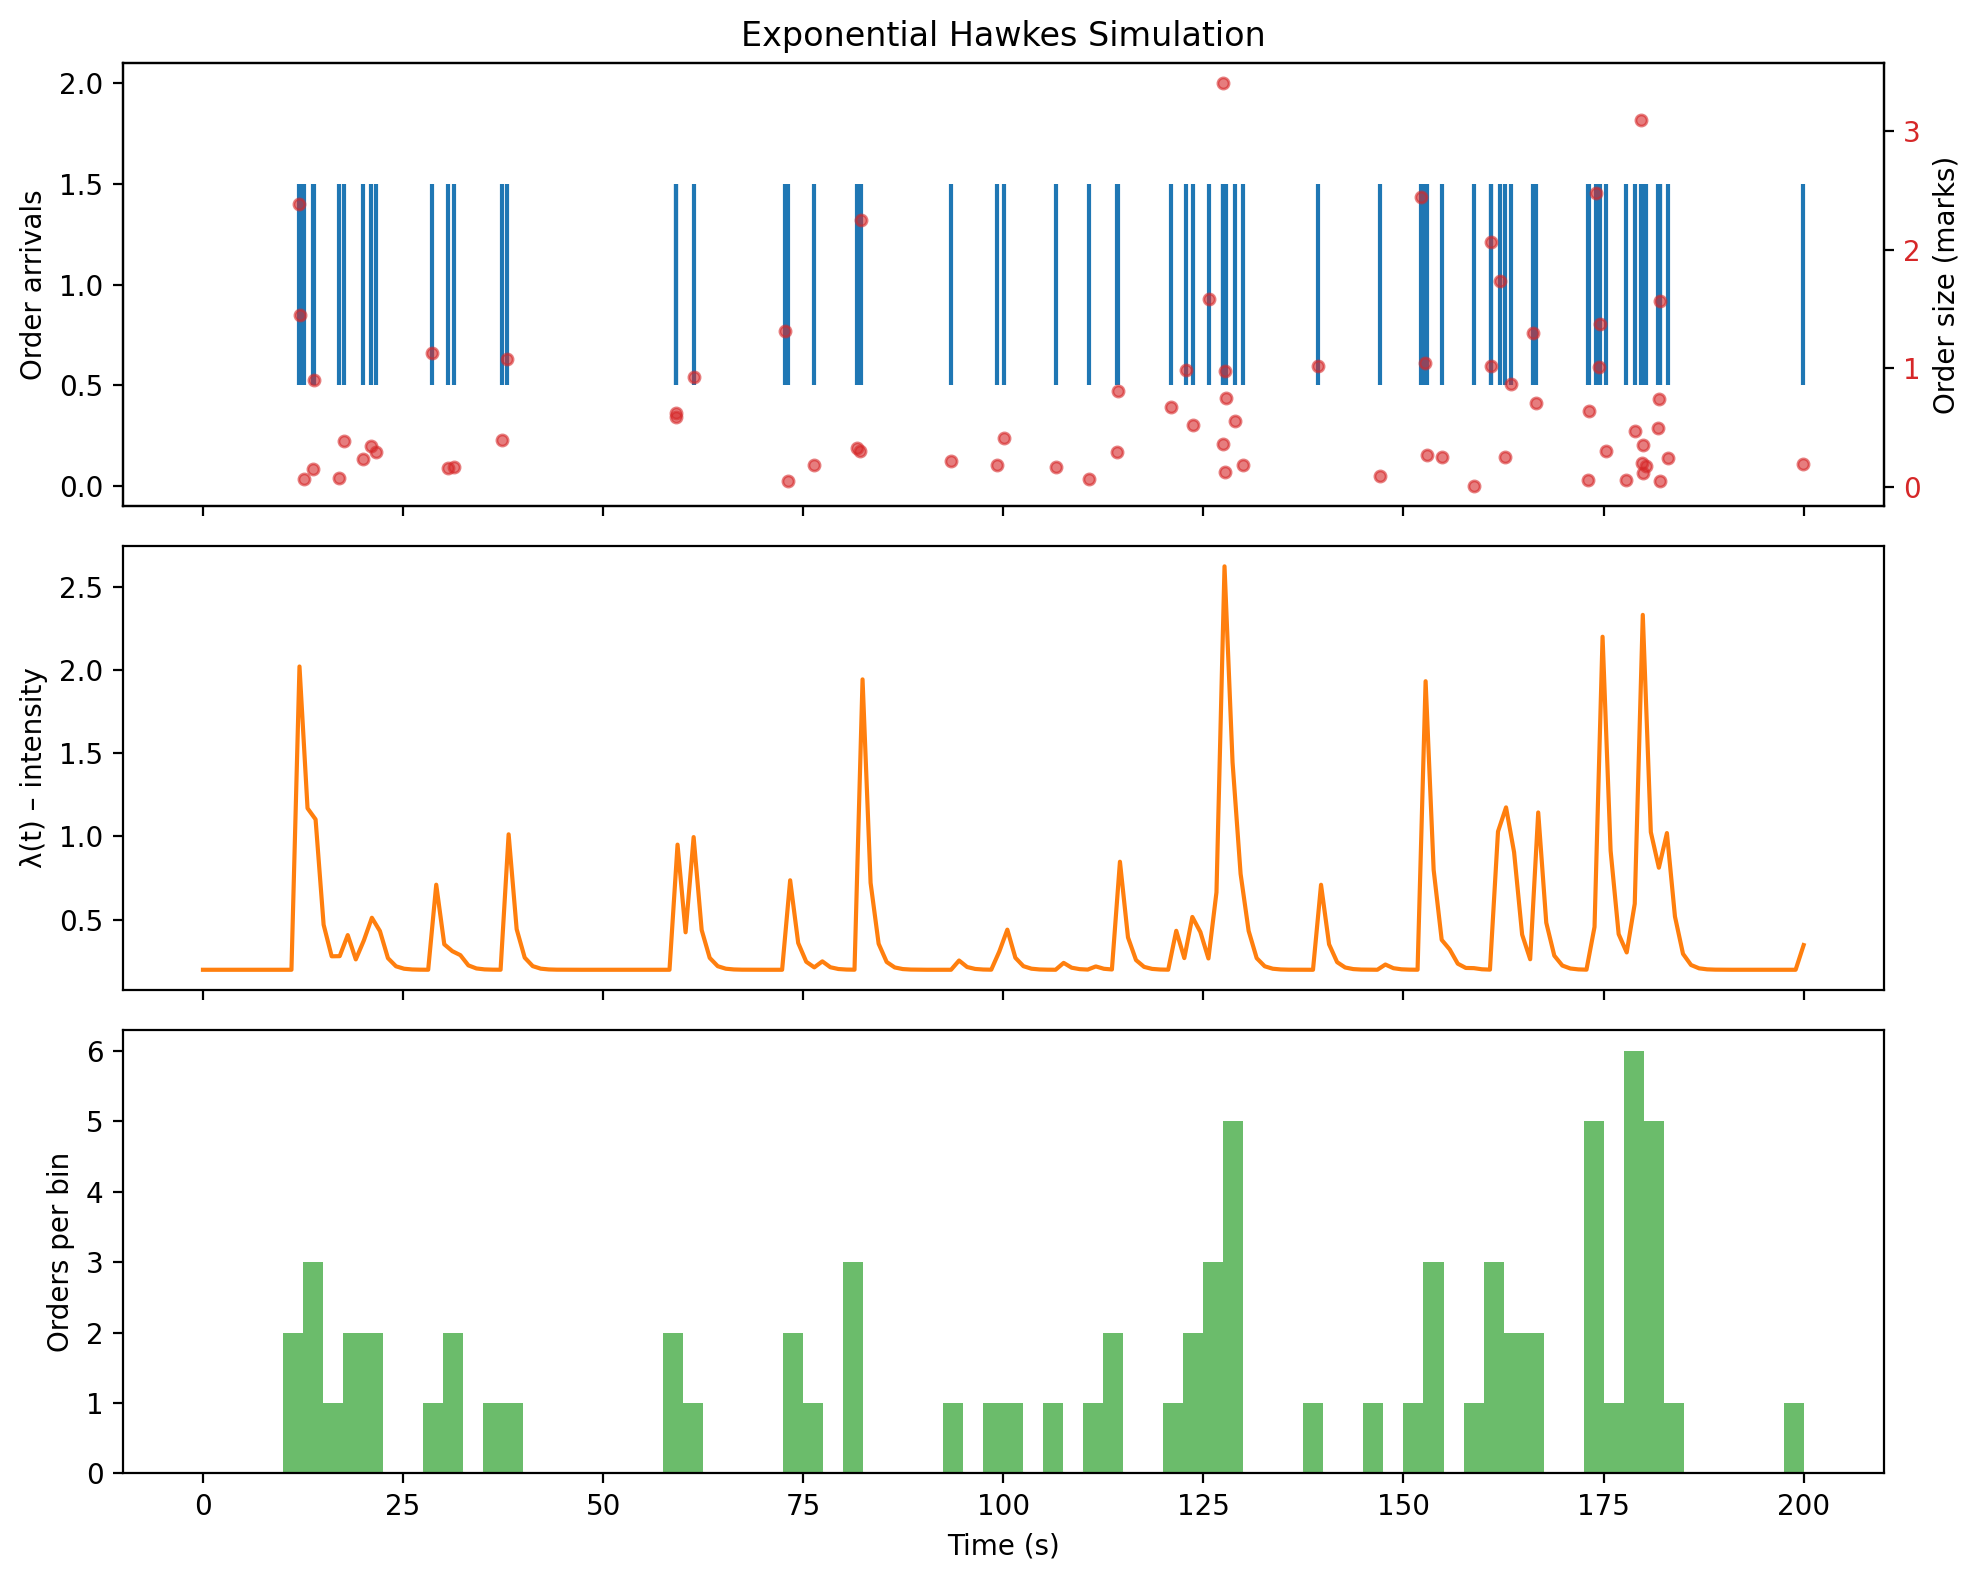
\includegraphics[width=0.9\linewidth]{../images/timeline_exponential.png}
  \caption{\textbf{Hawkes simulation timeline.} Event arrivals, marks, intensity $\lambda(t)$, and binned counts for the calibrated exponential kernel on Binance BTCUSDT. A power-law overlay (purple) is available via the released scripts.}
  \label{fig:timeline}
\end{figure}

\begin{figure}[H]
  \centering
  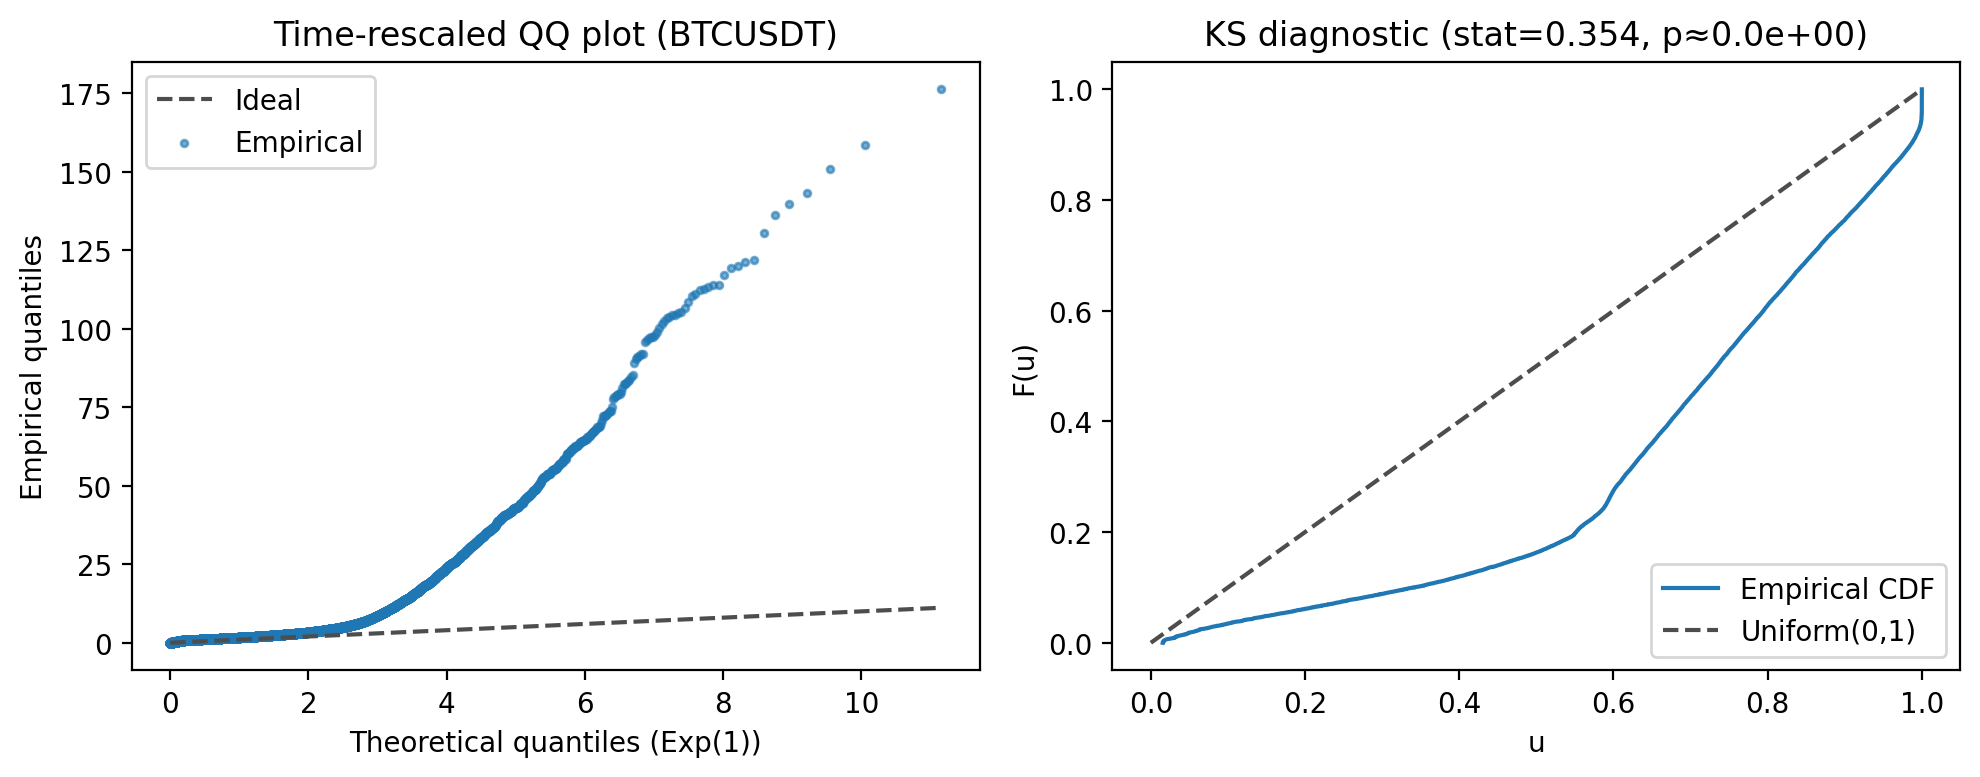
\includegraphics[width=0.9\linewidth]{../images/qq_ks_btcusdt.png}
  \caption{\textbf{Residual diagnostics.} Time-rescaling QQ plot (left) and KS empirical CDF (right) for the exponential kernel fit on Binance BTCUSDT. Deviations from the diagonal indicate under-dispersion of long gaps.}
  \label{fig:qqks}
\end{figure}

\begin{table}[t]
  \centering\small
  \begin{tabular}{lrrrr}
    \toprule
    Model & NLL $\downarrow$ & KS $\downarrow$ & ACF(1) & Est. branching $\hat{n}$ \\
    \midrule
    Exponential Hawkes              & 0.817 & 0.038 & 0.419 & 0.755 \\
    Power-law Hawkes               & 0.842 & 0.056 & 0.320 & 0.754 \\
    Queue-reactive (baseline)      & 1.146 & 0.697 & 0.283 & 0.000 \\
    \bottomrule
  \end{tabular}
  \caption{\textbf{Benchmark summary on Binance BTCUSDT (validation slice).} Metrics are computed on 200-second simulation horizons regenerated with the released seeds. NLL is per-event, KS is the supremum distance on rescaled uniforms, and ACF(1) measures lag-one autocorrelation of 0.5-second arrival bins.}
  \label{tab:benchmarks}
\end{table}

\paragraph{Interpretation.} \Cref{fig:timeline} shows that the exponential kernel produces bursty intensities aligned with large volume marks; power-law kernels yield similar clustering but heavier tails (see supplement). Residual diagnostics in \cref{fig:qqks} reveal systematic departures from the Exp(1) reference for long inter-arrivals, echoing the high KS statistics in \cref{tab:benchmarks}. The queue-reactive baseline, lacking self-excitation, underestimates clustering (high NLL, large KS) yet achieves lower lag-one ACF because it reacts to depth instead of history. Branching ratios near $0.75$ confirm we operate in a nearly-unstable yet subcritical regime.

\paragraph{Comparative analysis.} Power-law kernels marginally increase NLL relative to the exponential fit but modestly reduce ACF, signalling longer memory yet noisier likelihood optimisation. The deterministic queue-reactive baseline exhibits the poorest likelihood but remains informative for stress-testing hybrid designs.

\section{Discussion and limitations}\label{sec:discussion}
Hawkes-driven flows capture clustering and cross-excitation but do not condition on instantaneous queue state. Queue-reactive models excel at matching imbalance-sensitive metrics but miss history-dependent bursts. A promising hybrid direction is to modulate Hawkes base rates with queue-derived features, blending self-excitation with instantaneous state feedback. Computationally, power-law kernels are costlier due to historical summations; incremental data structures or neural surrogates \cite{MeiEisner2017,Zuo2020} may alleviate this. Our study focuses on one-day crypto and one-hour equity slices; broader cross-venue evaluations and confidence intervals (e.g., via block bootstrap) remain future work.

\section{Reproducibility checklist}\label{sec:repro}
\begin{itemize}[leftmargin=*, itemsep=2pt]
  \item \textbf{Code and configs.} Repository: \url{https://github.com/sohaibelkarmi/High-Frequency-Trading-Simulator}. Key scripts: \texttt{scripts/pack\_binance\_npz.py}, \texttt{scripts/preprocess\_lobster.py}, \texttt{experiments/run\_matrix.py}, \texttt{scripts/prepare\_summary\_assets.py}.
  \item \textbf{Data provenance.} Raw Binance trades \cite{BinanceData} and LOBSTER Level-X feeds \cite{LOBSTER}. Metadata JSON files store preprocessing flags, timestamps, and RNG seeds.
  \item \textbf{Environment.} Experiments executed on Apple M-series CPUs with Python 3.11, PyTorch 2.2, NumPy 1.26. \texttt{requirements.txt} freezes versions; CMake scripts log compiler versions.
  \item \textbf{Artifacts.} All figures (PNG) and tables (CSV/LaTeX) regenerate via \texttt{python scripts/prepare\_summary\_assets.py}. Diagnostic notebooks export additional plots for inspection.
\end{itemize}

\section{Conclusion}
We documented a theory-backed, reproducible stack for Hawkes-driven LOB simulation and validated it on public crypto and equity datasets. The framework offers a baseline for hybrid Hawkes plus queue-reactive research and invites extensions toward neural intensity models with explicit calibration tests.

\paragraph{Availability.} Code and artifacts: \url{https://github.com/sohaibelkarmi/High-Frequency-Trading-Simulator}

% --- Minimal hand-written bibliography with links (for arXiv) ----------
\begin{thebibliography}{99}\setlength{\itemsep}{2pt}

\bibitem{Bacry2015}
E.~Bacry, I.~Mastromatteo, J.-F.~Muzy.
Hawkes processes in finance.
\emph{Market Microstructure and Liquidity} 1(1), 2015.
Preprint: \url{https://arxiv.org/abs/1502.04592}.

\bibitem{BremaudMassoulie1996}
P.~Br\'{e}maud, L.~Massouli\'{e}.
Stability of nonlinear Hawkes processes.
\emph{Annals of Probability} 24(3):1563--1588, 1996.
Link: \url{https://projecteuclid.org/journals/annals-of-probability/volume-24/issue-3/Stability-of-nonlinear-Hawkes-processes/10.1214/aop/1065725193.full}.

\bibitem{JaissonRosenbaum2015}
T.~Jaisson, M.~Rosenbaum.
Limit theorems for nearly unstable Hawkes processes.
\emph{Annals of Applied Probability} 25(2), 2015.
Preprint: \url{https://arxiv.org/abs/1310.2033}.

\bibitem{ContLarrard2013}
R.~Cont, A.~de Larrard.
Price dynamics in a Markovian limit order market.
\emph{SIAM J. Financial Mathematics} 4(1), 2013.
Preprint: \url{https://arxiv.org/abs/1104.4596}.

\bibitem{HuangLehalleRosenbaum2015}
W.~Huang, C.-A.~Lehalle, M.~Rosenbaum.
Simulating and analyzing order book data: The queue-reactive model.
\emph{JASA} 110(509), 2015.
Preprint: \url{https://arxiv.org/abs/1312.0563}.

\bibitem{Ogata1981}
Y.~Ogata.
On Lewis' simulation method for point processes.
\emph{IEEE Trans. Info. Theory} 27(1):23--31, 1981.
PDF: \url{https://bemlar.ism.ac.jp/zhuang/Refs/Refs/ogata1981ieee.pdf}.

\bibitem{LewisShedler1979}
P.A.W.~Lewis, G.S.~Shedler.
Simulation of nonhomogeneous Poisson processes by thinning.
\emph{Naval Research Logistics Quarterly} 26(3):403--413, 1979.
DOI: \url{https://onlinelibrary.wiley.com/doi/10.1002/nav.3800260304}.

\bibitem{Brown2002}
E.N.~Brown, R.~Barbieri, V.~Ventura, R.E.~Kass, L.M.~Frank.
The time-rescaling theorem and its application to neural spike train data analysis.
\emph{Neural Computation} 14(2):325--346, 2002.
PDF: \url{https://stat.cmu.edu/~kass/papers/rescaling.pdf}.

\bibitem{DaleyVereJones2003}
D.~Daley, D.~Vere-Jones.
\emph{An Introduction to the Theory of Point Processes, Volume I}. Springer, 2003.

\bibitem{LOBSTER}
J.~Huang, M.~Polak, C.~Yueshen, et al.
LOBSTER: Limit Order Book Reconstruction System.
Info/Downloads: \url{https://lobsterdata.com/}.

\bibitem{BinanceData}
Binance public market data (trades, spot/futures) portal.
\url{https://data.binance.vision/}.

\bibitem{ContKukanovStoikov2014}
R.~Cont, A.~Kukanov, S.~Stoikov.
The price impact of order book events.
\emph{Journal of Financial Econometrics} 12(1):47--88, 2014.
Preprint: \url{https://arxiv.org/abs/1011.6402}.

\bibitem{GouldBonart2015}
M.D.~Gould, J.~Bonart.
Queue imbalance as a one-tick-ahead price predictor in a limit order book.
Preprint: \url{https://arxiv.org/abs/1512.03492}.

\bibitem{MollerRasmussen2005}
J.~M{\o}ller, J.G.~Rasmussen.
Perfect simulation of Hawkes processes.
\emph{Advances in Applied Probability} 37(3):629--646, 2005.
PDF: \url{https://www.cambridge.org/core/services/aop-cambridge-core/content/view/BCC3A80DEF4895F0E8F78A6716910AC8/S0001867800000392a.pdf}.

\bibitem{MeiEisner2017}
H.~Mei, J.~Eisner.
The neural Hawkes process: A neurally self-modulating approach to point process modeling.
In \emph{Advances in Neural Information Processing Systems}, 2017.
Preprint: \url{https://arxiv.org/abs/1612.09328}.

\bibitem{Zuo2020}
S.~Zuo, H.~Xu, L.~Sun, et al.
Transformer Hawkes process.
In \emph{International Conference on Machine Learning}, 2020.
Preprint: \url{https://arxiv.org/abs/2002.09291}.

\bibitem{Tick}
E.~Bacry, M.~Bompaire, L.~Ga"{i}ffas, S.~Poulenard.
Tick: a Python library for statistical learning, with a focus on time-dependent modelling.
\emph{Journal of Machine Learning Research} 18(214):1--5, 2018.
Preprint: \url{https://arxiv.org/abs/1707.03003}.

\end{thebibliography}

\end{document}
